\documentclass[paper=a4, fontsize=11pt]{article}
\usepackage[utf8]{inputenc}
\usepackage[english,magyar]{babel}
\usepackage{amsmath}
\usepackage{graphicx} 
\usepackage{float}
\usepackage{rotating}
\usepackage{latexsym}
\usepackage{listings}

\addtolength{\oddsidemargin}{-.875in}
\addtolength{\evensidemargin}{-.875in}
\addtolength{\textwidth}{1.95in}
\addtolength{\topmargin}{-.9in}
\addtolength{\textheight}{1.6in}

\begin{document}
\begingroup
	\centering
	\LARGE Szimuláció 1: Oszcillátor\\
\vspace{1 cm}
\large Nagy Péter\\
\large M07ILF\\
\vfill
\large 2018.03.12.\\

\newpage

\tableofcontents
\newpage


\section{Mérések}
A mérés során a mellékelt forráskód segítségével 4 különbőző paraméter esetében vizsgáltam a sztohasztikus rendszer viselkedését. A rugóállandót és a ugrások nagyságát egységnyinek vettem a szimulációban.
\newline
\flushleft
 A szimuláció paraméterei:

\begin{itemize}
  \item lépések száma: 10000
\item kezdő pozició: 0
\item a lépés hossza:1
\item a rugóállandó:1
\end{itemize}
  

\subsection{A lépések eloszlása}
Minden esetben megfigyelhető, hogy a lépések ugyanolyan valószinüséggel történnek.

\begin{figure}[h]
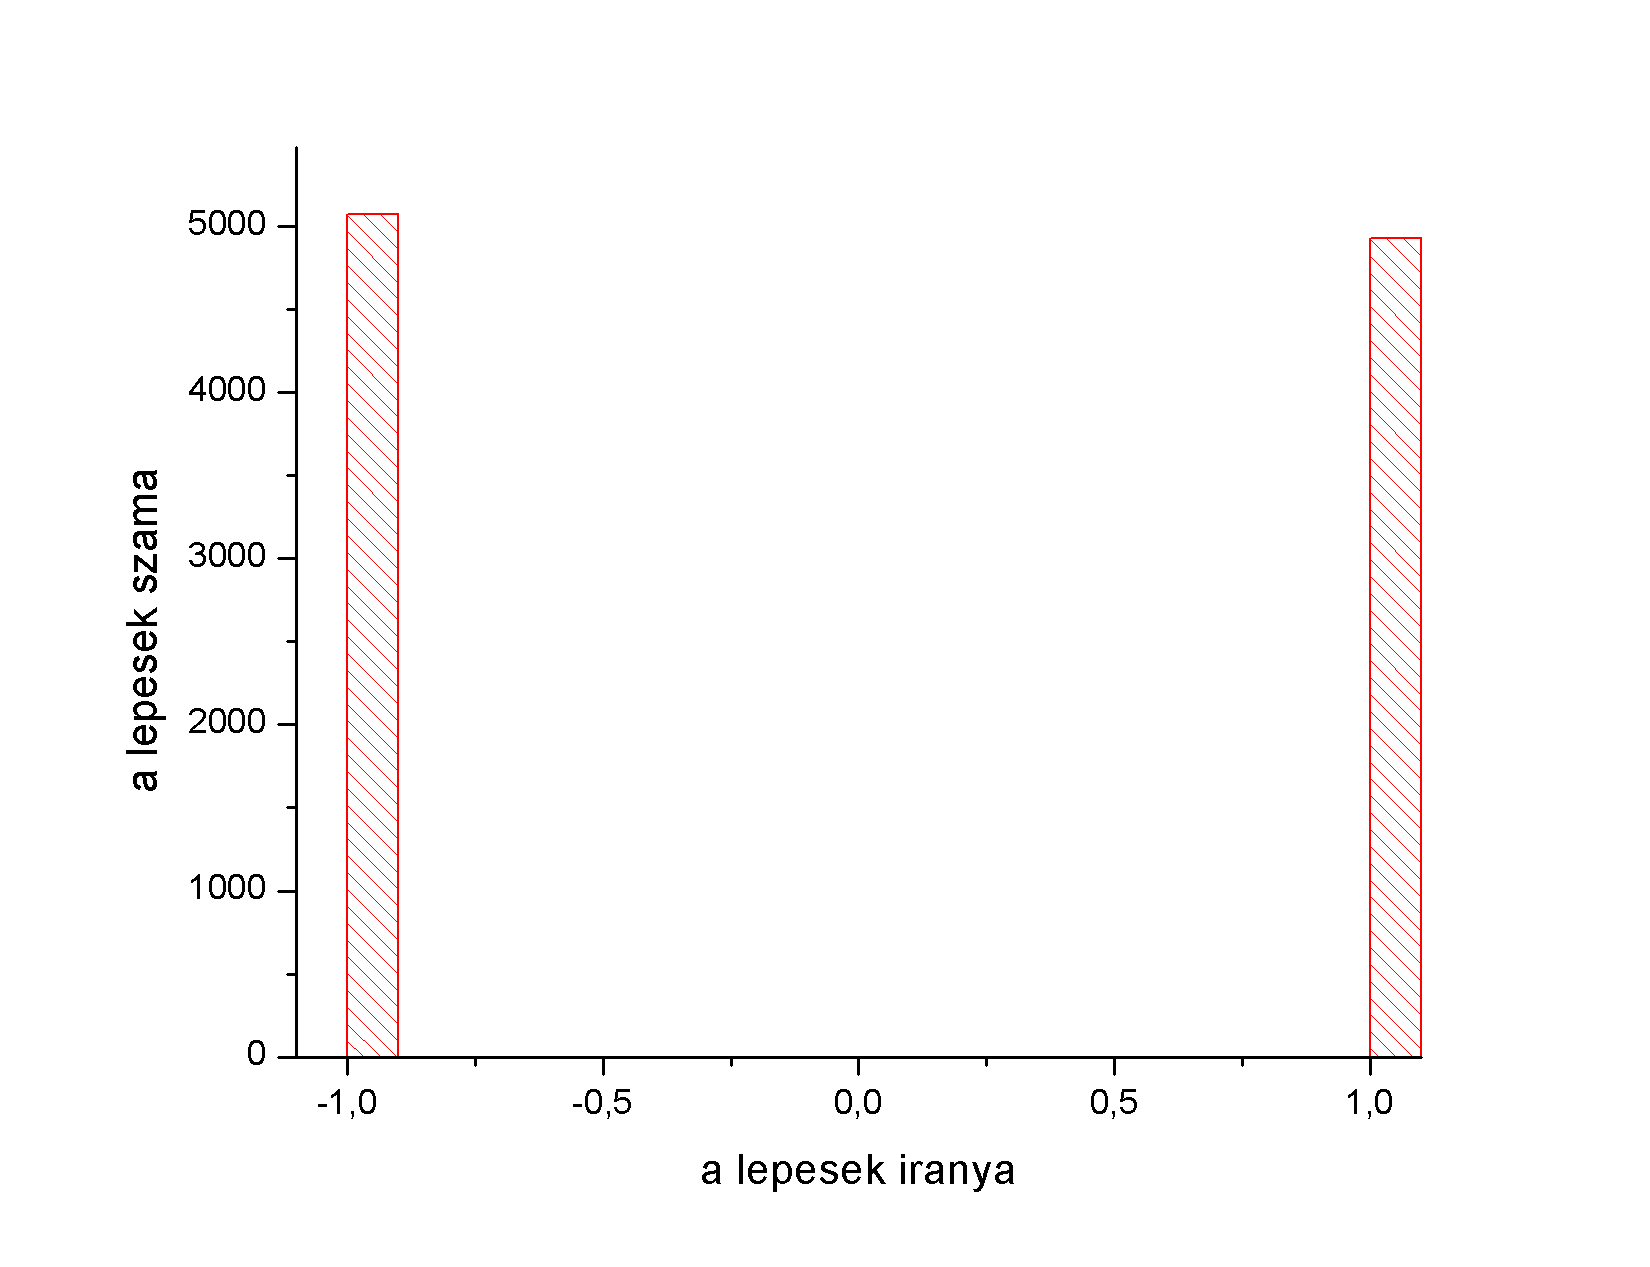
\includegraphics[width=\textwidth]{lep.png}
\caption{A lépések irányának eloszlása}
\end{figure}



\subsection{A mért adatok hisztogramjainak elemzése}

A megadott paraméter függvényében azt figyelhetjük meg, hogy ahogyan növeljük $\beta$ értékét, úgy egyre inkább nehezebben távolodik el a kiindulási ponttól a vizsgált részecske. Ez várható is volt, mert a szimulációs modelben a második elágazásnál azt a feltételt szabjuk, hogy a $e^{- \beta *\Delta E}$-nél kell kisebb véletlen számott huznunk a lépés végrehajtásához és ebben az esetben minnél nagyobb $\beta$ értéke annál valószinütlenebb, hogy a véletlen számunk kisebb lesz ennél a kifejezésnél.
Minden egyes mért adatsornál meghatározzuk a részecske koordinátájának az átlagos értékét (1) és a koordináta fluktuációját (4). 
Valamint meghatározzuk az egyensúlyi eloszlásfüggvényt. Azt figyeljük meg, hogy ahogyan csökken a $\beta$ paraméter úgy csökken az átlag értéke és a koordináta fluktuációja.
\begin{align}
&<x>= \frac{1}{N} \sum_{k=1}^N an_k\\
&<x>=a<n>\\
&<x^2>=a^2<n^2>\\
&<x^2>-<x>^2
\end{align}

\begin{figure}[H]
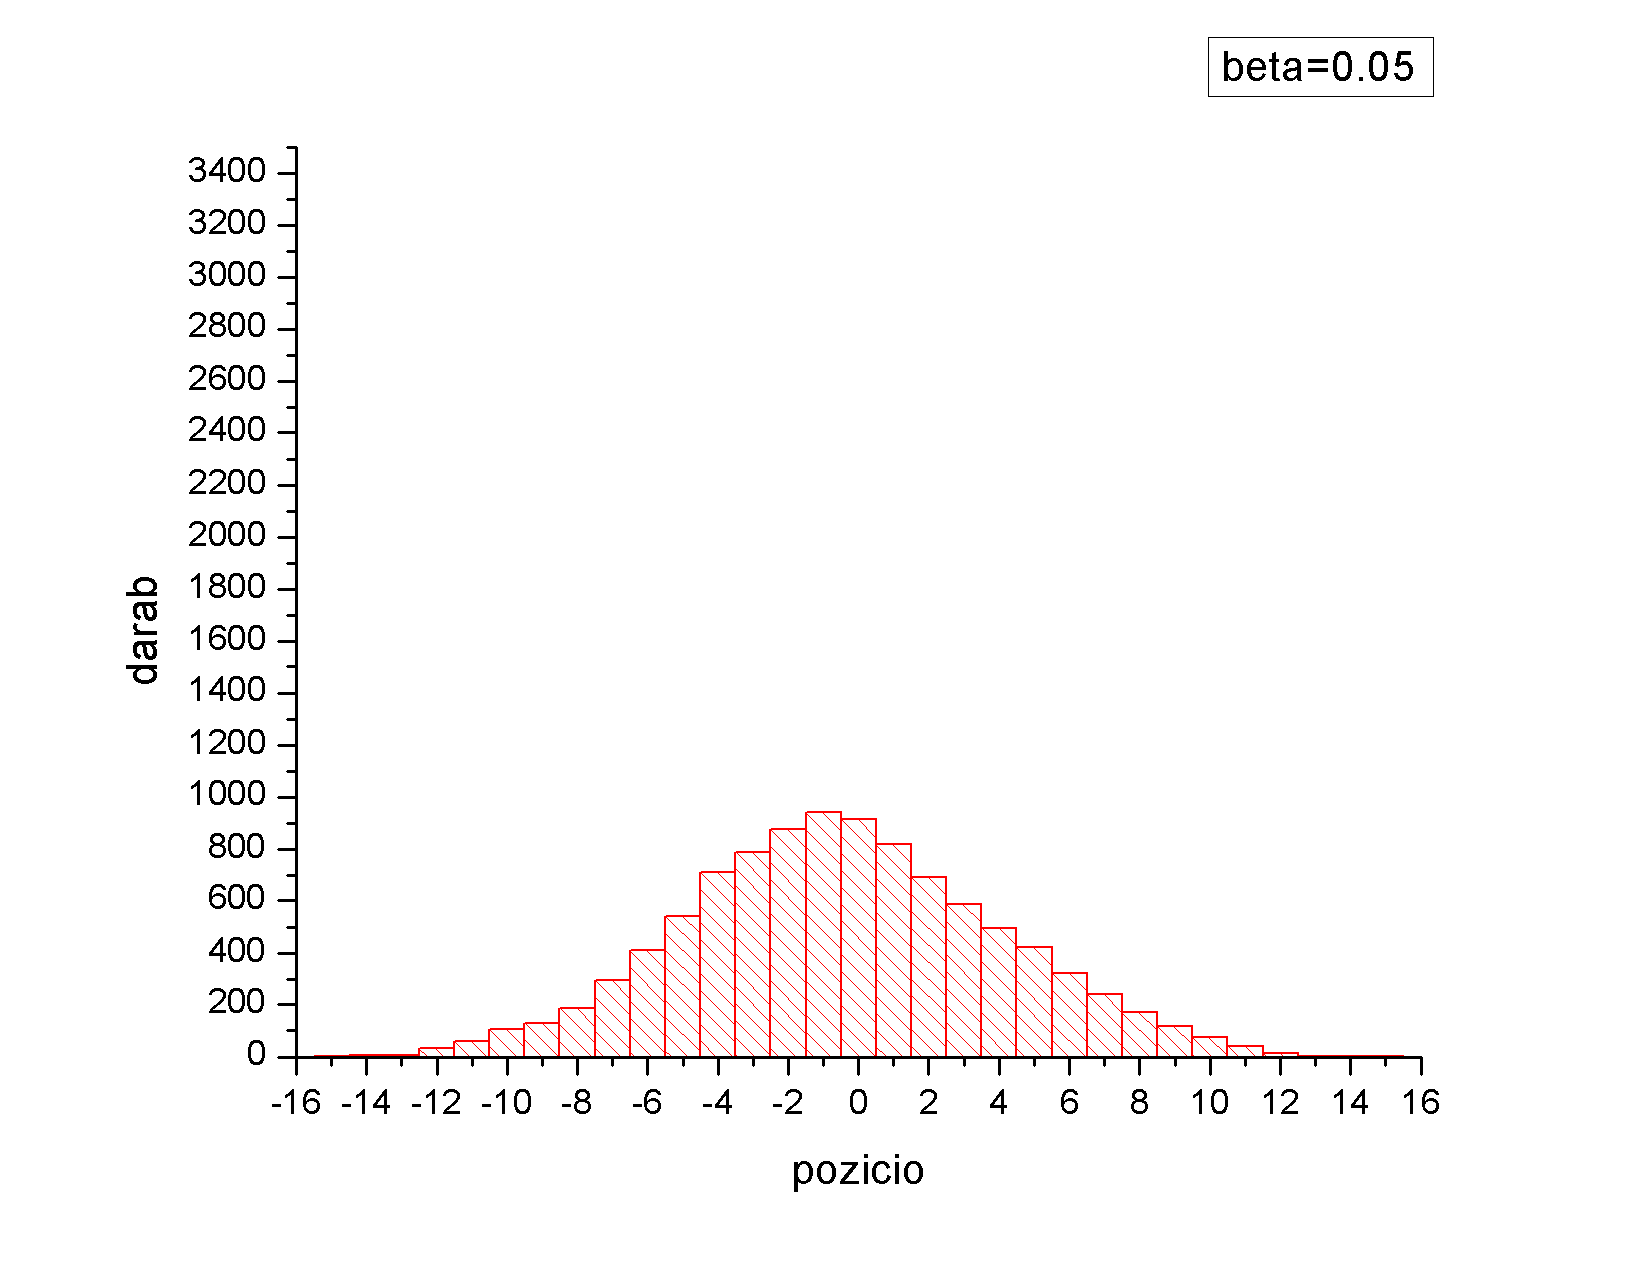
\includegraphics[width=\textwidth]{1.png}
\caption{Az elfoglalt helyzetek eloszlása}
\end{figure}

\begin{align}
&<x>= -0,45\\
&<x^2>=20\\
&<x^2>-<x>^2=19,78
\end{align}



\begin{figure}[H]
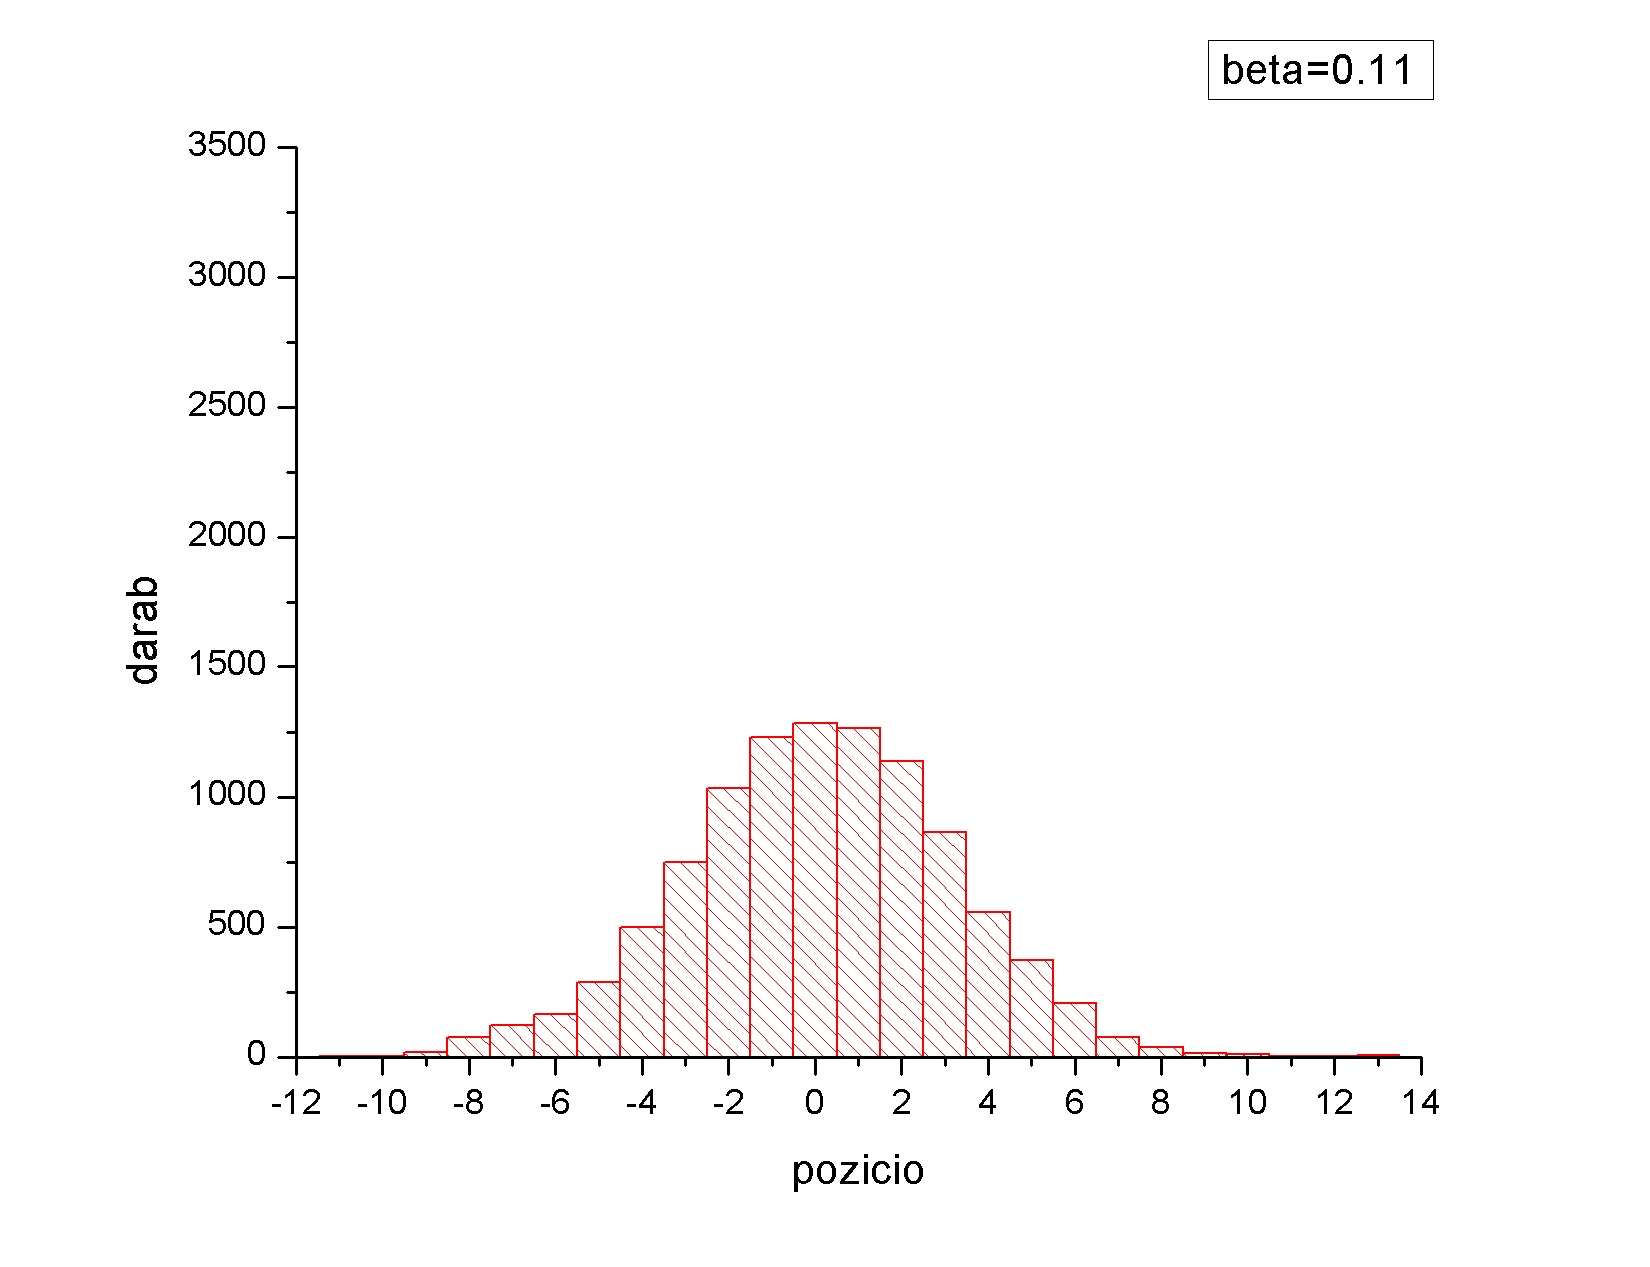
\includegraphics[width=\textwidth]{2.png}
\caption{Az elfoglalt helyzetek eloszlása}
\end{figure}

\begin{align}
&<x>= 0,11\\
&<x^2>=9,47\\
&<x^2>-<x>^2=9,47
\end{align}




\begin{figure}[H]
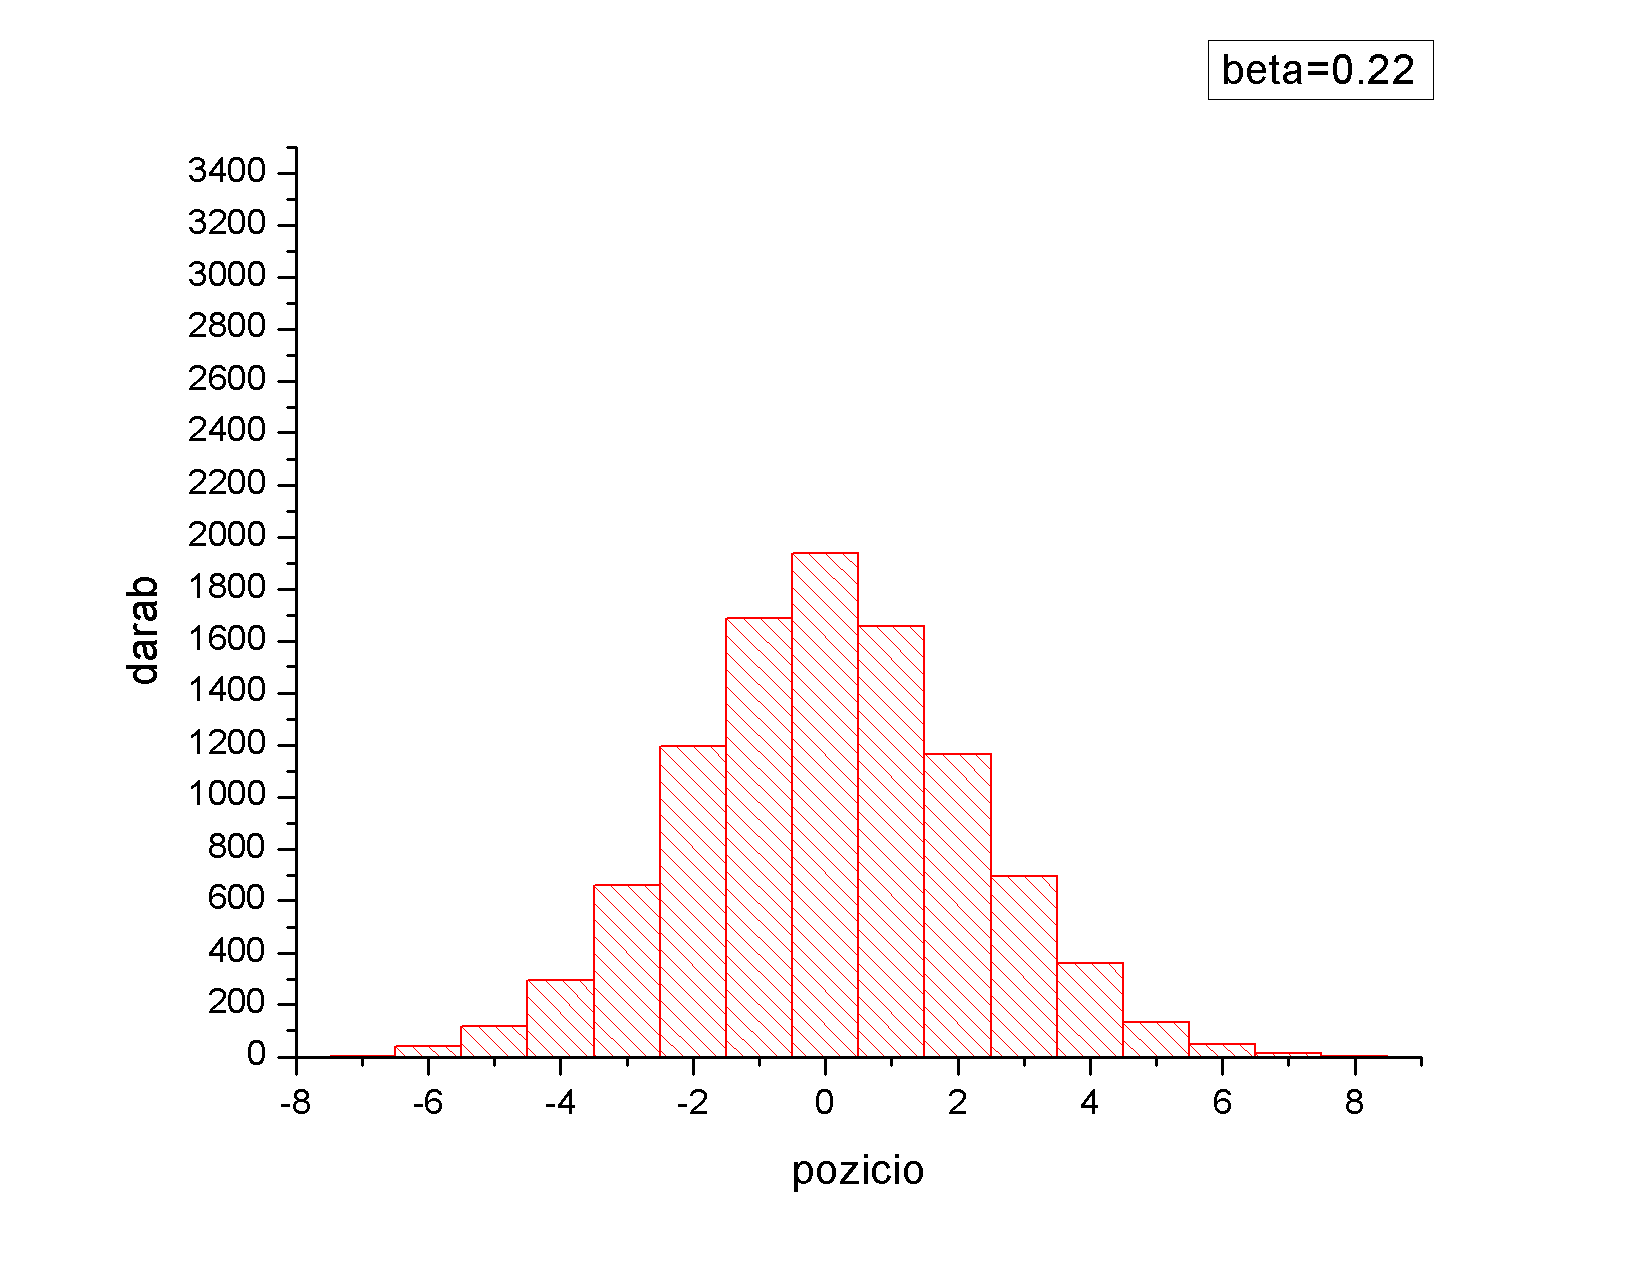
\includegraphics[width=\textwidth]{3.png}
\caption{Az elfoglalt helyzetek eloszlása}
\end{figure}


\begin{align}
&<x>= 0,05\\
&<x^2>=4,57\\
&<x^2>-<x>^2=4,56
\end{align}


\begin{figure}[H]
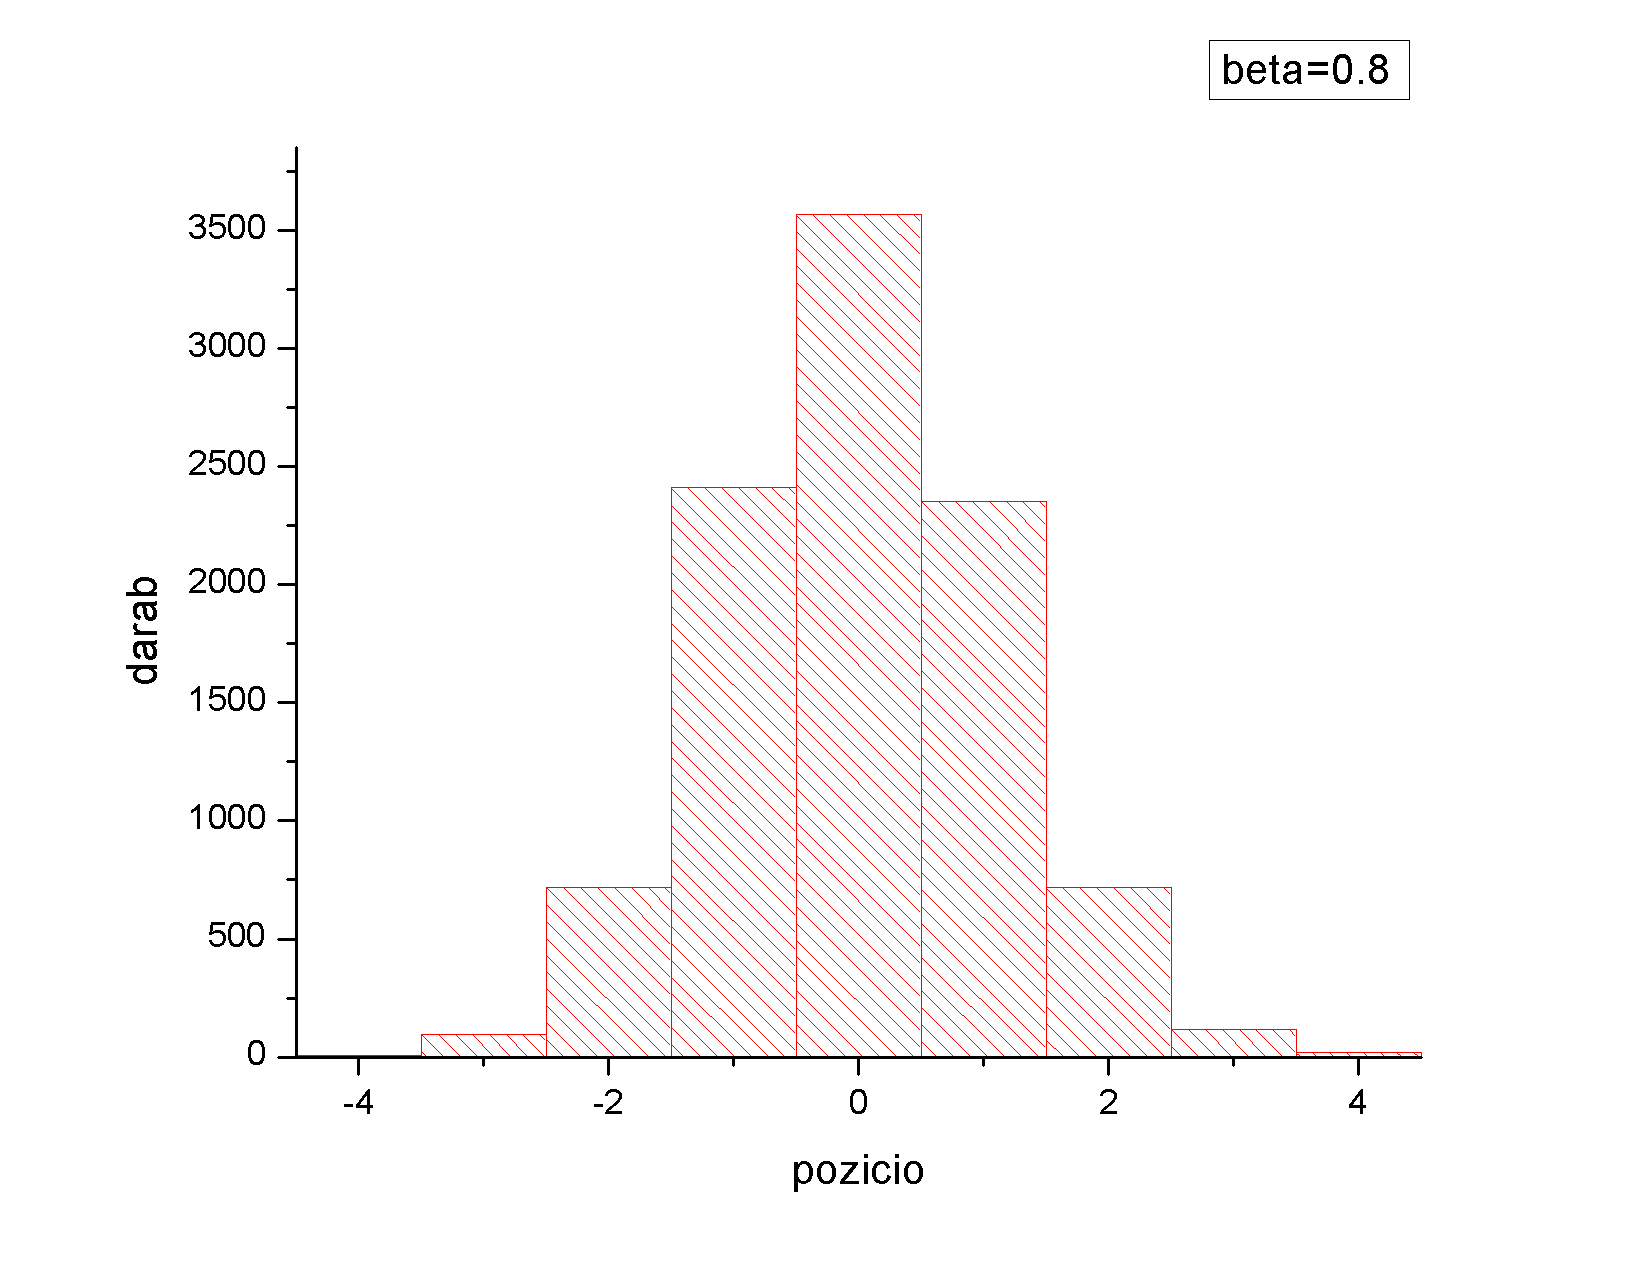
\includegraphics[width=\textwidth]{4.png}
\caption{Az elfoglalt helyzetek eloszlása}
\end{figure}


\begin{align}
&<x>= 0,01\\
&<x^2>=1,28\\
&<x^2>-<x>^2=1,28
\end{align}


\subsection{Eloszlás az egyensúlyi állapotban}
Az eloszlásról ránézésre megállapítható, hogy normális eloszlást követ az egyensúly állapotában.
\begin{align}
P^{(e)}(n)=\frac{1}{\beta \sqrt{2\pi}}e^{-\frac{(x-m)^2}{2 \beta^2}}
\end{align}
Ahol $\beta$ a megadott paraméter és m a kiindulási pont.

\begin{figure}[H]
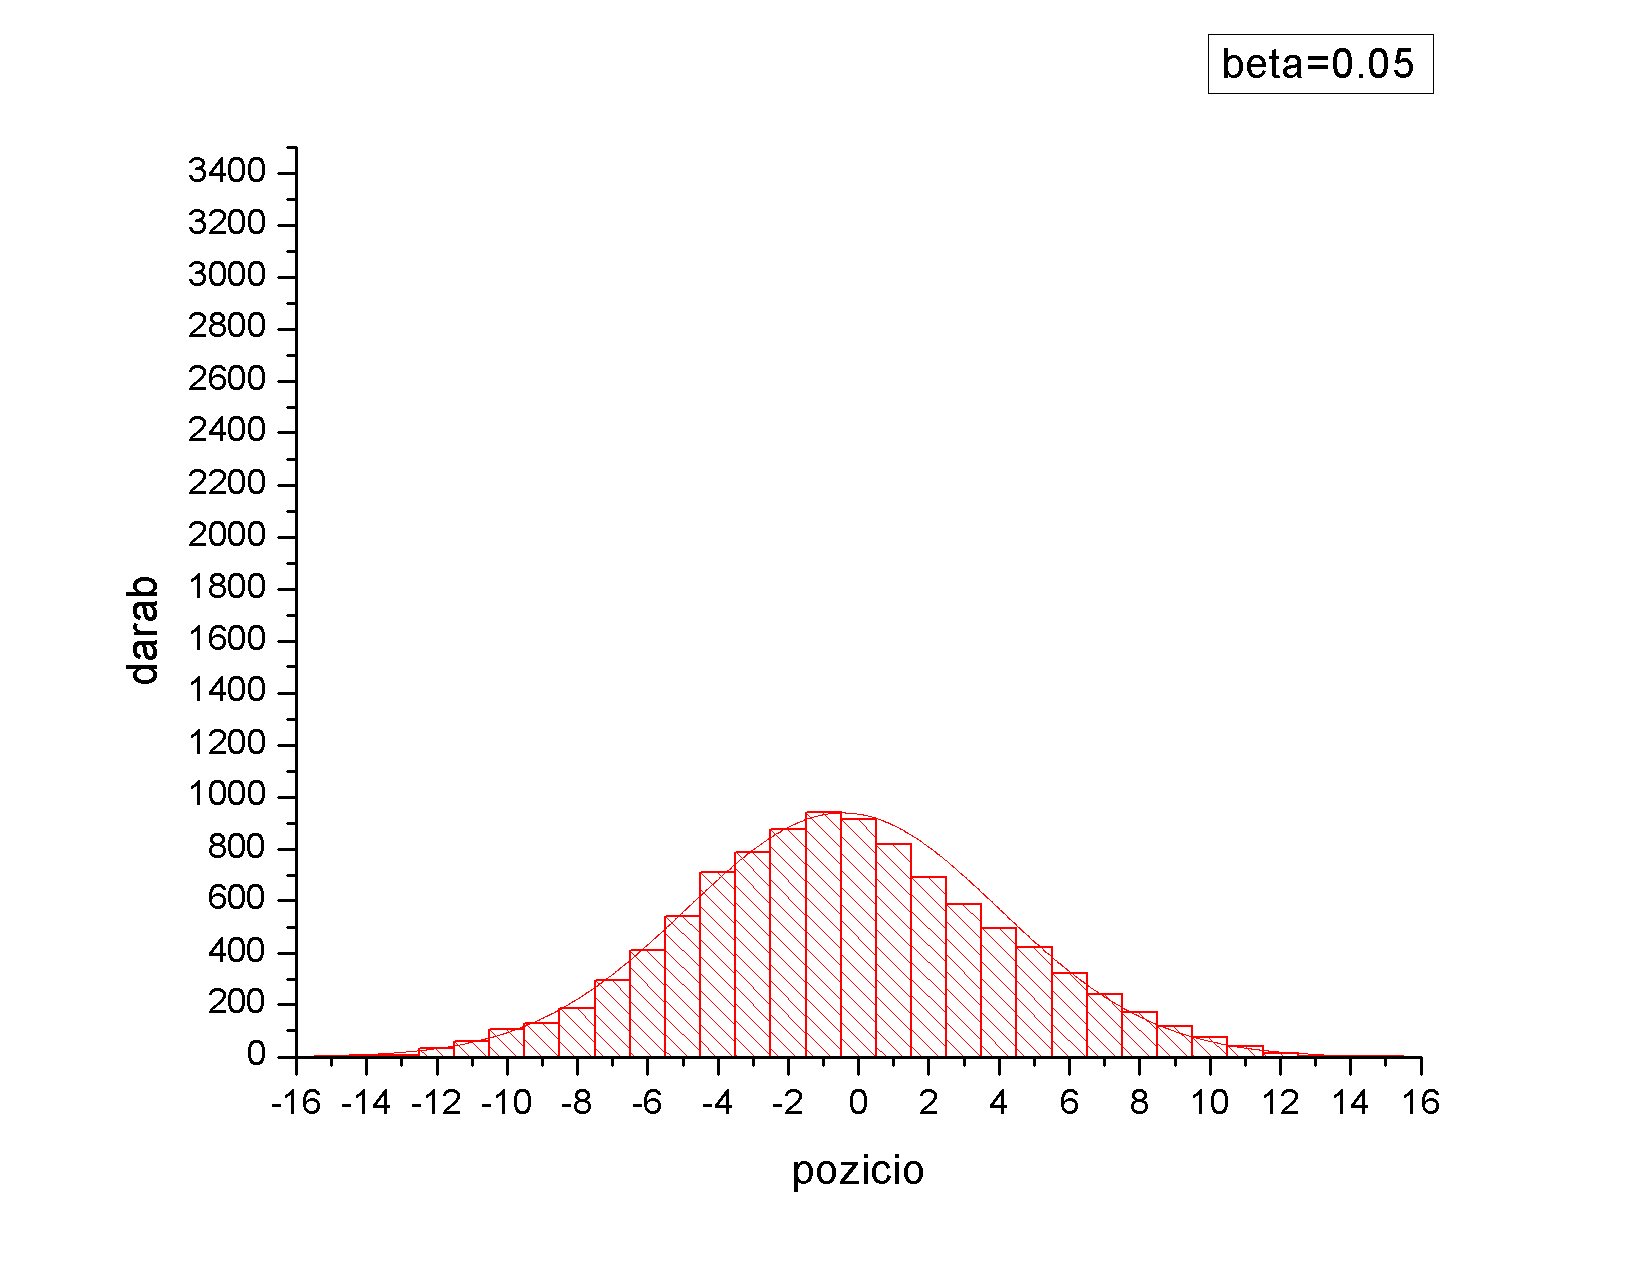
\includegraphics[width=\textwidth]{1g.png}
\caption{Az illesztett gauss görbe}
\end{figure}
\begin{figure}[H]
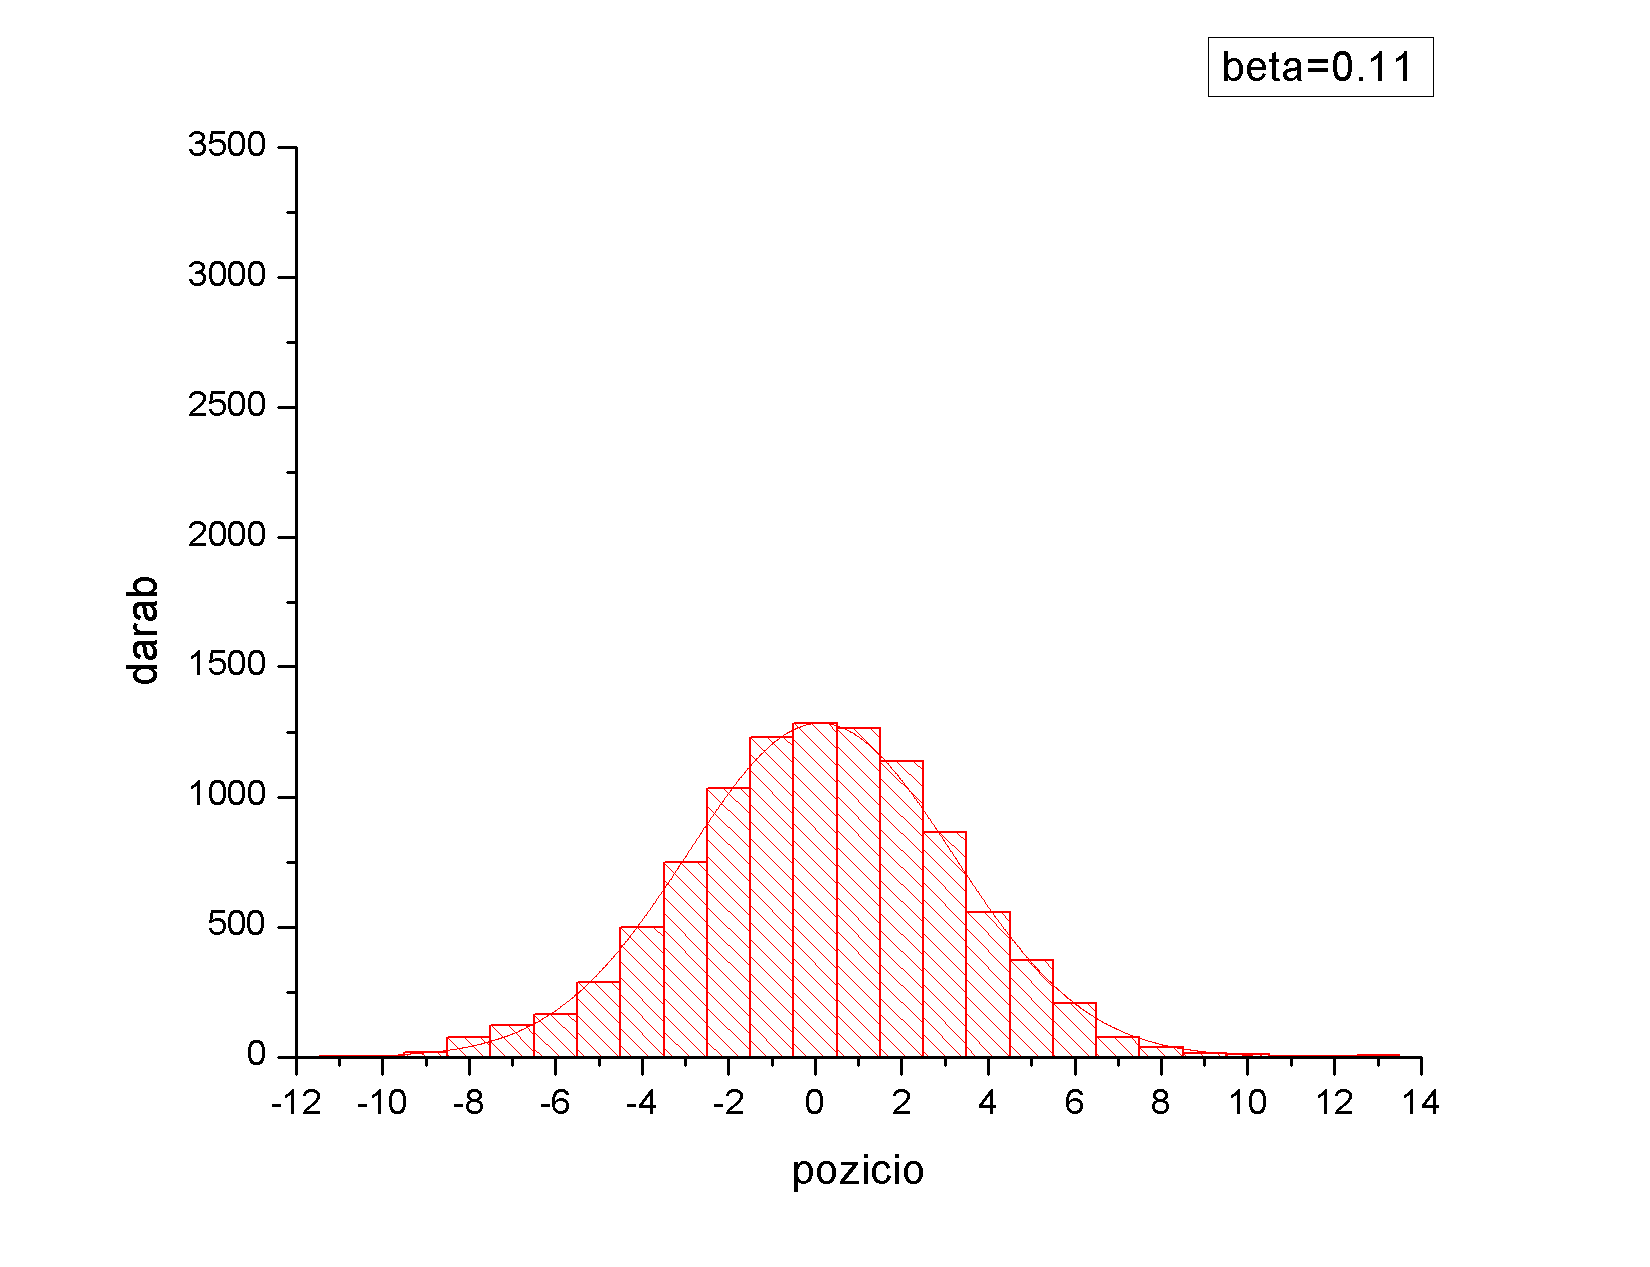
\includegraphics[width=\textwidth]{2g.png}
\caption{Az illesztett gauss görbe}
\end{figure}
\begin{figure}[H]
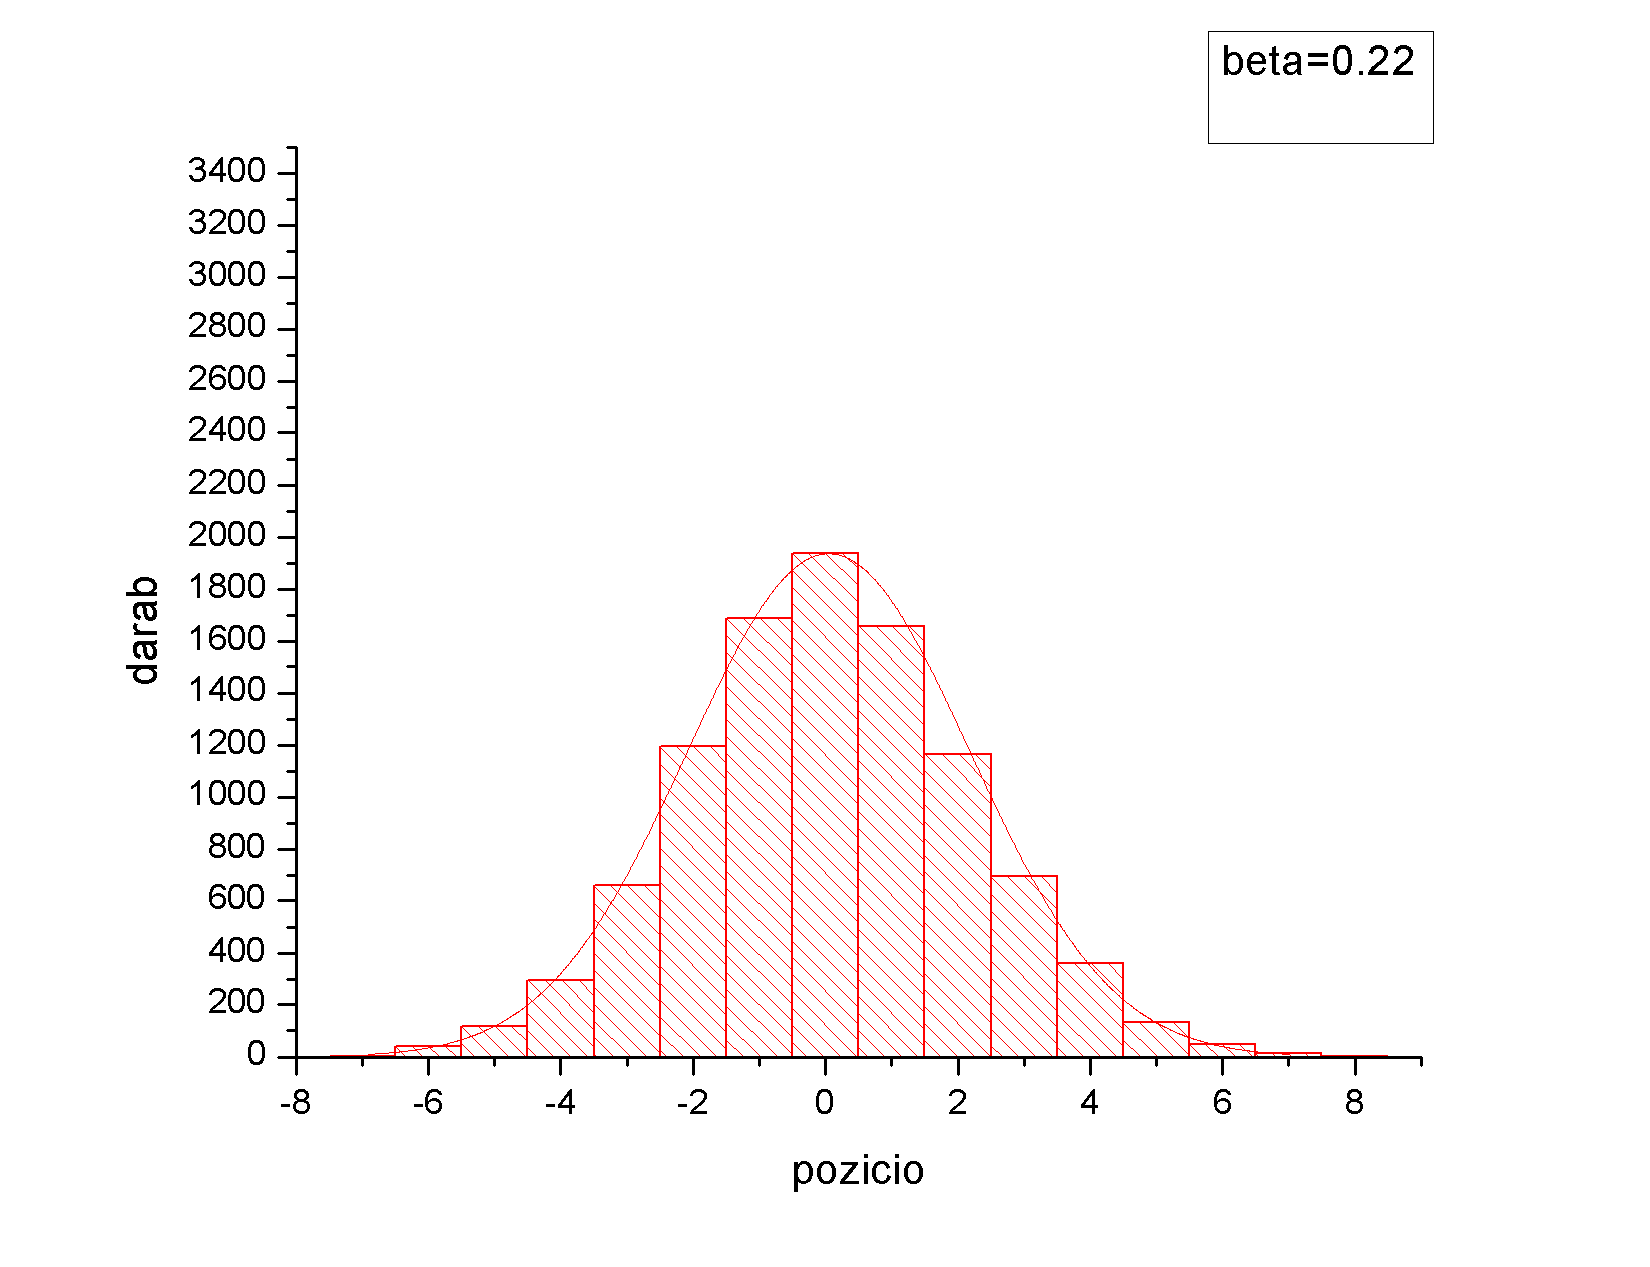
\includegraphics[width=\textwidth]{3g.png}
\caption{Az illesztett gauss görbe}
\end{figure}
\begin{figure}[H]
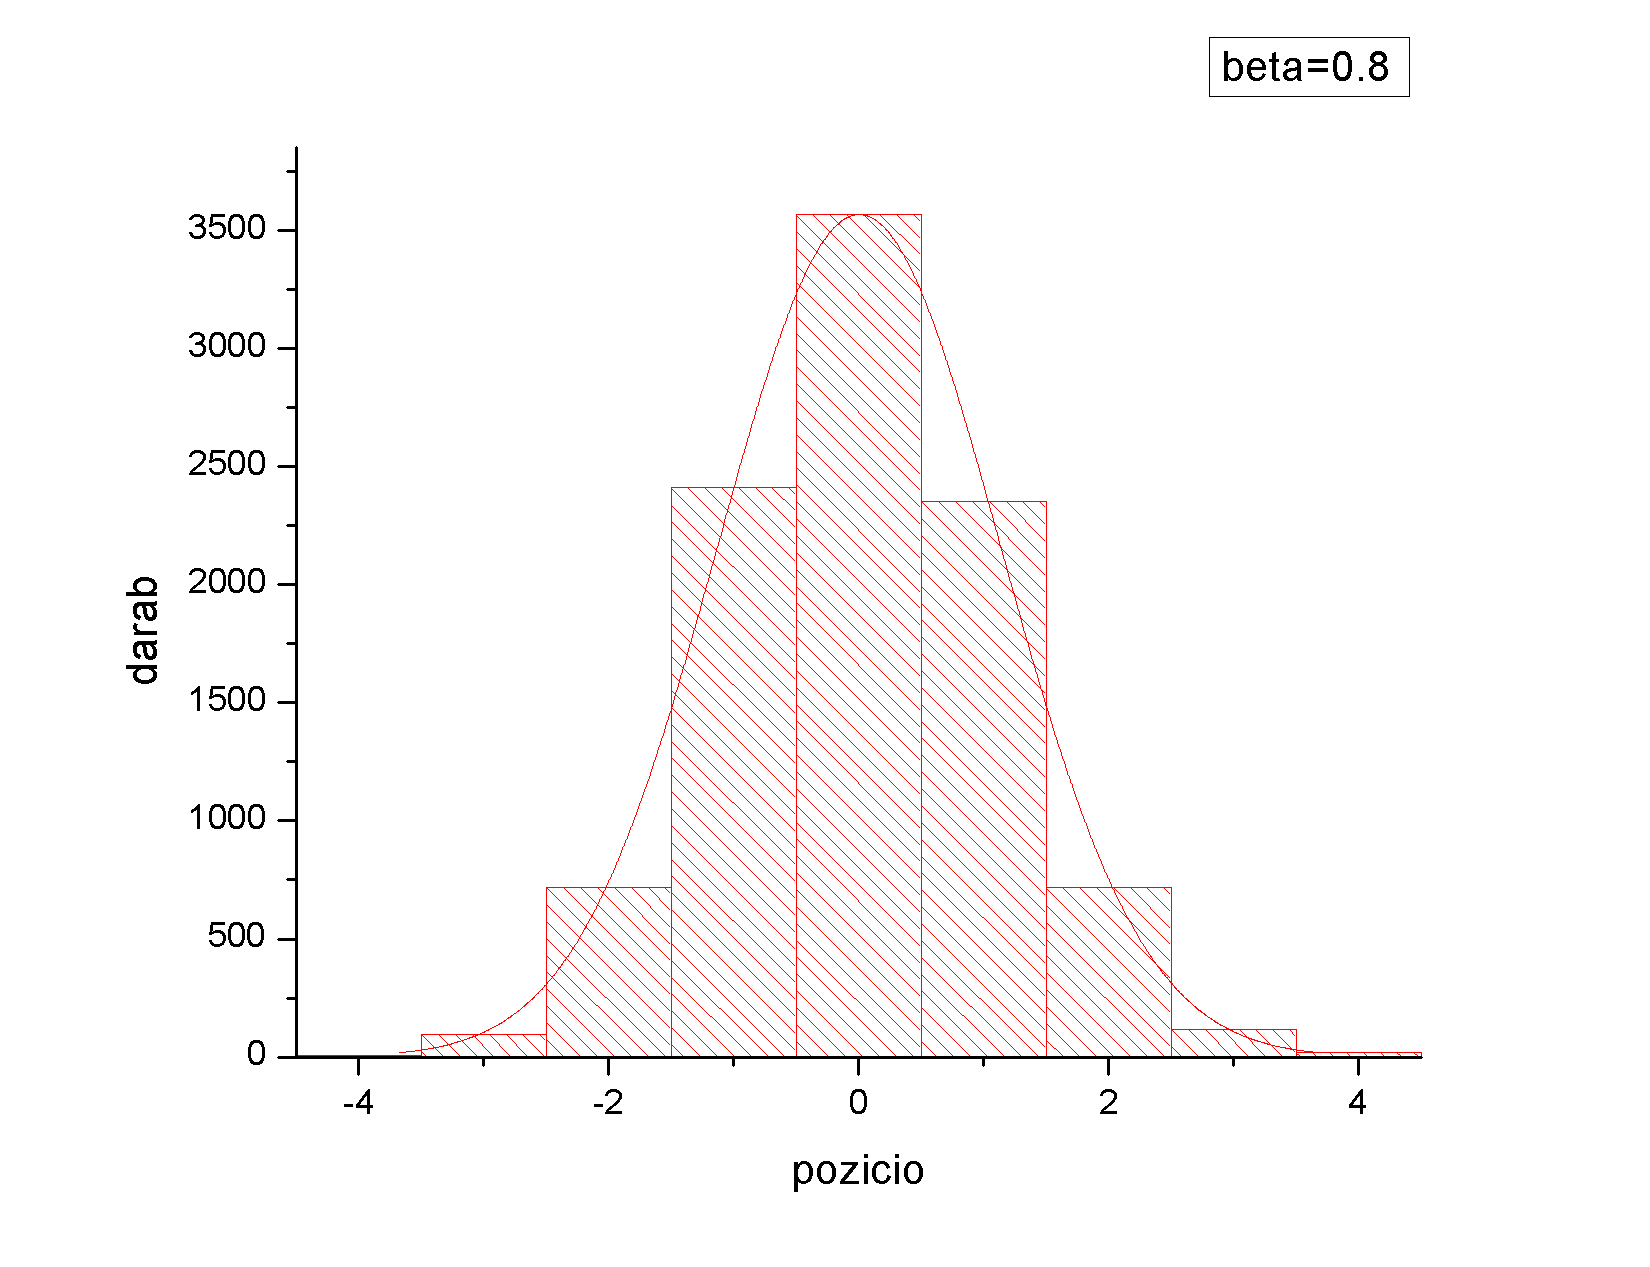
\includegraphics[width=\textwidth]{4g.png}
\caption{Az illesztett gauss görbe}
\end{figure}

 \end{document}























\end{document}